\begin{name}
	{\tenchude}
	{\tendethi}
	{\tentruong}
	{\thoigian}
\end{name}
\Opensolutionfile{ansbook}[ans/ansbook-3]
\TN
\Opensolutionfile{ans}[ans/ans-3-T]
\begin{ex}%Câu 1
	Hàm số $y=f(x)$ có đồ thị như sau. Hàm số $y=f(x)$ đồng biến trên khoảng nào dưới đây?\\
	\centerline{
		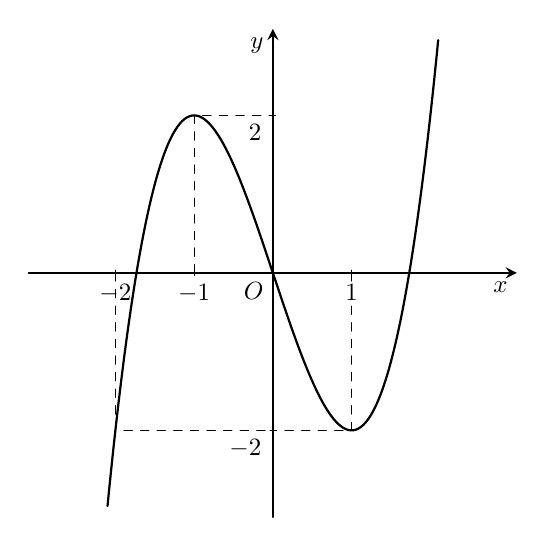
\begin{tikzpicture}[line join=round, line cap=round,>=stealth,thick]
			\tikzset{every node/.style={scale=0.9}}
			\draw[->] (-3.1,0)--(3.1,0) node[below left] {$x$};
			\draw[->] (0,-3.1)--(0,3.1) node[below left] {$y$};
			\draw (0,0) node [below left] {$O$};
			\foreach \x/\nx in {-2/-2,-1/-1,1/1}
			\draw[thin] (\x,1pt)--(\x,-1pt) node [below] {$\nx$};
			\foreach \y/\ny in {-2/-2,2/2}
			\draw[thin] (1pt,\y)--(-1pt,\y) node [below left] {$\ny$};
			\draw[dashed,thin](-2,0)--(-2,-2)--(0,-2);
			\draw[dashed,thin](1,0)--(1,-2)--(0,-2);
			\draw[dashed,thin](-1,0)--(-1,2)--(0,2);
			\begin{scope}
				\clip (-3,-3) rectangle (3,3);
				\draw[samples=200,domain=-2.1:2.1,smooth,variable=\x] plot (\x,{1*((\x)^3)+0*((\x)^2)+-3*(\x)+0});
			\end{scope}
		\end{tikzpicture}
	}
	\choice
	{\True $\left(-2;-1\right)$}
	{$\left(-1;1\right)$}
	{$\left(-2;1\right)$}
	{$\left(-1;2\right)$}
	\loigiai{
		Từ đồ thị, hàm số đã cho đồng biến trên khoảng $\left(-2;-1\right)$ .}
\end{ex}
\begin{ex}%Câu 2
	Trong không gian với hện tọa độ $Oxyz$ , cho mặt cầu $(S):{x^2}+y^2+z^2-2x+4y+6z-2=0$ . Bán kính của mặt cầu $(S)$ bằng:
	\choice
	{8}
	{12}
	{\True 4}
	{16}
	\loigiai{
		Mặt cầu $(S)$ có tâm $I\left(1\,;\,-2\,;\,-3\right)$ và có bán kính $R=\sqrt{1+4+9-\left(-2\right)}=\sqrt{16}=4$}
\end{ex}
\begin{ex}%Câu 3
	Tiệm cận ngang của đồ thị hàm số $y=\dfrac{1-2x}{x-2}$ là đường thẳng:
	\choice
	{$y=1$}
	{$x=2$}
	{\True $y=-2$}
	{$x=-2$}
	\loigiai{
		Đường tiệm cận ngang của đồ thị hàm số là: $y=\dfrac{a}{c}=-\dfrac{2}{1}=-2$ .}
\end{ex}
\begin{ex}%Câu 4
	Tìm tập nghiệm $S$ của bất phương trình $\log_{\tfrac{1}{2}}\left(x-3\right)\ge\log_{\tfrac{1}{2}}4$ .
	\choice
	{\True $S=\left(3;7\right]$}
	{$S=\left[3;7\right]$}
	{$S=\left(-\infty ;7\right]$}
			{$S=\left[7;+\infty\right)$}
	\loigiai{
		$\log_{\tfrac{1}{2}}\left(x-3\right)\ge\log_{\tfrac{1}{2}}4\Leftrightarrow 0<x-3\le 4\Leftrightarrow 3<x\le 7$ (vì $0<\dfrac12<1$).\\
		Vậy tập nghiệm của bất phương trình là: $S=\left(3;7\right]$}
\end{ex}
\begin{ex}%Câu 5
	Trong không gian $Oxyz$, một vectơ chỉ phương của đường thẳng $d\colon \heva{&x=-t+2\\&    y=2t\\&    z=3t}$ là
	\choice
	{$\left(2;2;3\right)$}
	{$\left(1;2;3\right)$}
	{\True $\left(1;-2;-3\right)$}
	{$\left(2;-2;-3\right)$}
	\loigiai{
		Một vectơ chỉ phương của đường thẳng $d$ là $\overrightarrow{u_d}=\left(-1\,;\,2\,;\,3\right)$}
\end{ex}
\begin{ex}%Câu 6
	Cho hình chóp $S.ABCD$ có đáy $ABCD$ là hình chữ nhật, cạnh $AB=a,BC=2a$ . Hai mặt bên $\left(SAB\right)$ và ($SAD)$ cùng vuông góc với mặt phẳng $\left(ABCD\right)$ và cạnh $SA=a$ . Tính theo $a$ thể tích $V$ của khối chóp $S.ABCD$
	\choice
	{$V=a^3$}
	{\True $V=\dfrac{2a^3}{3}$}
	{$V=2a^3$}
	{$V=\dfrac{a^3}{3}$}
	\loigiai{
		Ta có: $SA\perp\left(ABCD\right)$ và $SA=a$\\
		Thể tích khối chóp $S.ABCD$ là: $V_{S.ABCD}=\dfrac{1}{3} \cdot a \cdot a \cdot 2a=\dfrac{2a^3}{3}$}
\end{ex}
\begin{ex}%Câu 7
	Hàm số $y=3^{x^2+1}$ có giá trị nhỏ nhất bằng
	\choice
	{$1$}
	{$5$}
	{\True $3$}
	{$0$}
	\loigiai{
		Ta thấy: $x^2+1\ge 1$ và dấu \lq\lq =\rq\rq~ xảy ra khi $x=0$ nên $3^{x^2+1}\ge{3^1}=3$}
\end{ex}
\begin{ex}%Câu 8
	Cho hàm số $f(x)=x^2-\dfrac{4}{x}$. Giá trị của $\displaystyle\int\limits_1^2 f'(x)\mathrm{\,d}x$ bằng
	\choice
	{$\dfrac{7}{3}- \ln 2$}
	{$3$}
	{$\dfrac{7}{3}$}
	{\True $5$}
	\loigiai{
		Ta có: $\displaystyle\int\limits_1^2f'(x)\mathrm{\,d}x= f(x)\vert_1^2=f(2)-f(1)=\left(2^2-\dfrac{4}{2}\right)-\left(1^2-\dfrac{4}{1}\right)=5$
	}
\end{ex}
\begin{ex}%Câu 9
	Cho một cấp số cộng có số hạng đầu là $u_1=2$ và công sai $d=3$ . Số hạng thứ 10 bằng:
	\choice
	{\True 29}
	{32}
	{26}
	{30}
	\loigiai{
		Ta có: $u_{10}=u_1+9d=2+9.3=2+27=29$}
\end{ex}
\begin{ex}%[Nguyễn Tuấn, dự án sáng tác đề 12]%[2D4N3-1]
	\immini{Diện tích phần hình phẳng gạch chéo trong hình vẽ bên được tính theo công thức nào dưới đây?
		\choice
		{$\displaystyle\int\limits_{-1}^2\left(2x^2-2x-4\right)\mathrm{\,d}x$}
		{$\displaystyle\int\limits_{-1}^2(-2x+2)\mathrm{\,d}x$}
		{$\displaystyle\int\limits_{-1}^2(2x-2)\mathrm{\,d}x$}
		{\True $\displaystyle\int\limits_{-1}^2\left(-2x^2+2x+4\right)\mathrm{\,d}x$}}
	{\begin{tikzpicture}[scale=.7, font=\footnotesize, line join=round, line cap=round, >=stealth]
			\draw[->] (-1.5,0) -- (3,0)node[below]{\footnotesize $x$};
			\draw (-1,0) circle (.5pt)node[below]{\footnotesize $-1$};
			\draw (2,0) circle (.5pt)node[above]{\footnotesize $2$};
			\draw[->,color=black] (0,-2.5) -- (0,3.5)node[below left]{\footnotesize $y$};
			\fill[pattern=north west lines] plot[smooth,samples=100,domain=-1:2] (\x,{(\x)^2-2*(\x)-1})--plot[smooth,samples=100,domain=2:-1] (\x,{-(\x)^2+3});
			\draw[thick,smooth,samples=100,domain=-1.5:2.2] plot(\x,{-(\x)^2+3});
			\draw[thick,smooth,samples=100,domain=-1.2:3] plot(\x,{(\x)^2-2*(\x)-1});
			\draw[dashed] (2,0) -- (2,-1) (-1,0) -- (-1,2);
			\filldraw[fill=white] (0,0) circle (1pt)node[shift={(-45:6pt)}]{\footnotesize $O$};
			\draw (2,3) node{\footnotesize $y=-x^2+3$};
			\draw (-1,-2.2) node{\footnotesize $y=x^2-2x-1$};
		\end{tikzpicture}}
	\loigiai{
		$S=\displaystyle\int\limits_{-1}^2\left[\left(-x^2+3\right)-\left(x^2-2x-1\right)\right]\mathrm{\,d}x=\displaystyle\int\limits_{-1}^2\left(-2x^2+2x+4\right)\mathrm{\,d}x$.
	}
\end{ex}
\begin{ex}%Câu 11
	Trong không gian với hệ tọa độ $Oxyz$ , cho điểm $M\left(3;5;-7\right)$ . Tìm tọa độ của điểm $M'$ đối xứng với điểm $M$ qua trục $Oy$ .
	\choice
	{$M'\left(3;-5;-7\right)$}
	{$M'\left(3;5;7\right)$}
	{$M'\left(-3;5;-7\right)$}
	{\True $M'\left(-3;5;7\right)$}
	\loigiai{
		Gọi $H$ là hình chiếu của $M$ lên $Oy$ nên suy ra $H\left(0\,;\,5\,;\,0\right)$\\
		Điểm $M'$ là điểm đối xứng với $M$ qua $H$ nên $M'=2H-M=\left(-3\,;\,5\,;\,7\right)$}
\end{ex}
\begin{ex}%Câu 12
	Một công ty thống kê lương của nhân viên theo tuần (đơn vị: USD) theo bảng sau:
	\begin{center}
		\begin{tabular}{|c|c|c|c|c|c|}
			\hline
			Lương theo tuần (USD) & $[10; 20)$ & $[20; 30)$ & $[30; 40)$ & $[40; 50)$ & $[50; 60]$ \\
			\hline
			Số công nhân          & 4          & 6          & 10         & 20         & 10         \\
			\hline
		\end{tabular}
	\end{center}
	Độ lệch chuẩn của mẫu số liệu này bằng bao nhiêu? (làm tròn tới hàng phần chục)
	\choice
	{\True 11,7}
	{12}
	{11,4}
	{12,5}
	\loigiai{
		Ta có: $n=50$\\
		Khi đó: $\overline{x}=\dfrac{1}{50}\left(4.15+6.25+10.35+20.45+10.55\right)=40,2$\\
		Phương sai của mẫu số liệu: $s^2=\dfrac{1}{50}\left(4.15^2+6.25^2+10.35^2+20.45^2+10.55^2\right)-\overline{x}^2=136,96$\\
		Độ lệch chuẩn của mẫu số liệu là: $s=\sqrt{s^2}=\sqrt{136,96}\approx 11,7$}
\end{ex}
\Closesolutionfile{ans}
\TNTF
\Opensolutionfile{ans}[ans/ans-3-TF]
\begin{ex}%Câu 13
	Cho hàm số $y=f(x)=ax+b-\dfrac{1}{x+c}$ có đồ thị như hình vẽ.\\
	\centerline{
		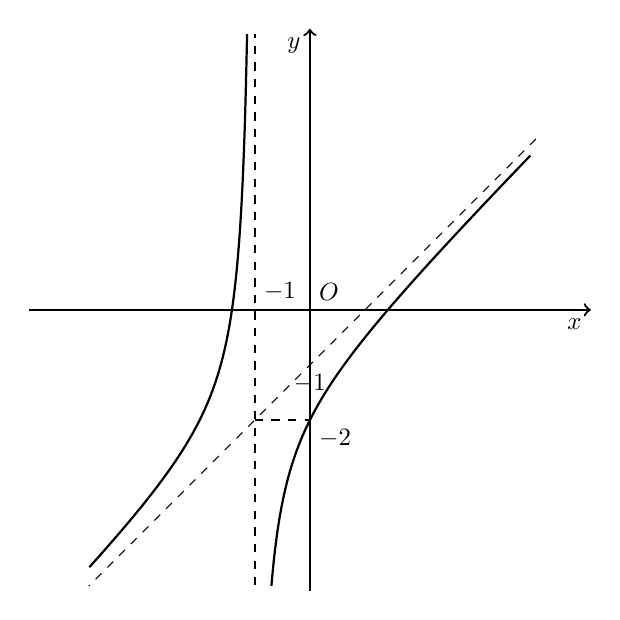
\begin{tikzpicture}[thick,scale=.7]
			\tikzset{every node/.style={scale=0.9}}
			\draw[->] (-5.1,0)--(5.1,0) node[below left] {$x$};
			\draw[->] (0,-5.1)--(0,5.1) node[below left] {$y$};
			\draw (0,0) node [above right] {$O$};
			\draw[dashed] (-0.99,-5)--(-0.99,5)
			(-1,-2)--(0,-2);
			\path
			(-1,0) node[above right]{$-1$}
			(0,-2)node[below right]{$-2$}
			(0,-1)node[below]{$-1$}
			;
			\begin{scope}
				\clip (-5,-5) rectangle (5,5);
				\draw[samples=200,domain=-4:-1.01,smooth,variable=\x] plot (\x,{(1*((\x)^2)+0*(\x)+-2)/(1*(\x)+1)});
				\draw[samples=200,domain=-0.99:4,smooth,variable=\x] plot (\x,{(1*((\x)^2)+0*(\x)+-2)/(1*(\x)+1)});
				\draw[dashed,thin] (-4.1,-5.1)--(4.1,3.1);
			\end{scope}
		\end{tikzpicture}
	}
	\choiceTF
	{Đồ thị hàm số nhận đường $x=-1$ làm tiệm cận đứng và đường $y=-x-1$ làm tiệm cận xiên}
	{\True Tâm đối xứng của đồ thị hàm số là điểm có tọa độ $\left(-1;-2\right)$}
	{\True $a+b+c=1$}
	{Gọi $I$ là tâm đối xứng của đồ thị hàm số và $M$ là 1 điểm bất kì thuộc đồ thị. Giá trị nhỏ nhất của độ dài đoạn thẳng $IM$ bằng $2\left(\sqrt{2}-1\right)$}
	\loigiai{
		a) Sai: Tiệm cận xiên của đồ thị hàm số có dạng $y=ax+b$ đi qua $\left(0\,;\,-1\right)$ và $\left(-1\,;\,-2\right)$ nên suy ra $\left\{\begin{aligned}
				 & a=1  \\
				 & b=-1 \\
			\end{aligned}\right.$ nên đường tiệm cận xiên là $y=x-1$\\
		Tiệm cận đứng là đường thẳng $x=-1\Leftrightarrow x=-c\Rightarrow-c=-1\Rightarrow c=1$\\
		b) Đúng: Từ đồ thị ta thấy tâm đối xứng của đồ thị hàm số là điểm có tọa độ $\left(-1;-2\right)$\\
		c) Đúng: $a+b+c=1+\left(-1\right)+1=1$.\\
		d) Sai: Dễ thấy $I\left(-1\,;\,-2\right)$ và hàm số ban đầu là $f(x)=x-1-\dfrac{1}{x+1}$ nên $M\left(x;\,x-1-\dfrac{1}{x+1}\right)$ với mọi $x\ne-1$ .\\
		Xét biểu thức $I{M^2}=\left(x+1\right)^2+\left[x-1-\dfrac{1}{x+1}-\left(-2\right)\right]^2=\left(x+1\right)^2+\left(x+1-\dfrac{1}{x+1}\right)^2$\\
		$=2\left(x+1\right)^2+\dfrac{1}{\left(x+1\right)^2}-2\ge 2\sqrt{2\left(x+1\right)^2.\dfrac{1}{\left(x+1\right)^2}}-2=2\sqrt{2}-2$ (Bất đẳng thức Cauchy)\\
		Vậy $IM=\sqrt{2\left(\sqrt{2}-1\right)}$ .}
\end{ex}
\begin{ex}%Câu 14
	Một nghệ nhân muốn làm một bình gốm có dạng mô hình như hình 2 bằng cách quay hình phẳng $(H)$ ở hình 1 quanh trục hoành. Biết đường cong trong hình 1 là phần đồ thị $y=0,125x^3$ trên đoạn $\left[0;2\right]$ và mỗi đơn vị trên đồ thị ở hình 1 có độ dài bằng 10 cm.\\
	\centerline{
		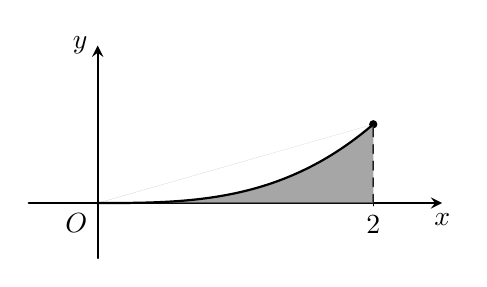
\begin{tikzpicture}[line join=round, line cap=round,>=stealth,thick,declare function={hs(\x)=0.125*((\x)^3);},x=1.75cm]
			\draw[->] (-.5,0)--(2.5,0) node[below] {$x$};
			\draw[->] (0,-.7)--(0,2) node[left] {$y$};
			\draw (0,0) node [below left] {$O$};
			\foreach \x/\nx in {2/2}
			\draw[thin] (\x,1pt)--(\x,-1pt) node [below] {$\nx$};
			\draw[dashed] (2,0)--(2,1);
			\fill (2,1) circle(1.5pt);
			\fill[gray,opacity=.7](0,0)--(2,0)--(2,1) plot[samples=200,domain=2:0,smooth](\x,{hs(\x)});
			\draw[samples=200,domain=0:2,smooth] plot (\x,{hs(\x)});
		\end{tikzpicture}
		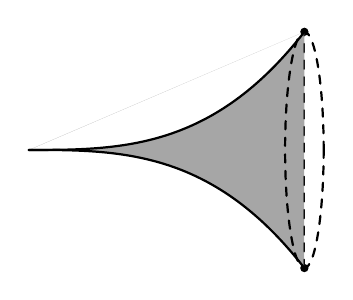
\begin{tikzpicture}[line join=round, line cap=round,>=stealth,thick,declare function={hs(\x)=0.125*((\x)^3);},x=1.75cm,y=1.5cm]
			\draw[dashed] (2,-1)--(2,1);
			\fill (2,1) circle(1.5pt) (2,-1) circle(1.5pt);
			\fill[gray,opacity=.7] plot[samples=200,domain=2:0,smooth](\x,{hs(\x)}) plot[samples=200,domain=0:2,smooth](\x,{hs(-\x)})--(2,1);
			\draw[samples=200,domain=0:2,smooth] plot (\x,{hs(\x)});
			\draw[samples=200,domain=0:2,smooth] plot (\x,{hs(-\x)});
			\draw[dashed] (2,0) ellipse (0.14 and 1);
		\end{tikzpicture}
	}
	\choiceTF
	{\True Chiều cao của bình gốm bằng 20 cm}
	{Đường kính đáy của bình gốm bằng 10 cm}
	{Khi cắt bình gốm bởi 1 mặt phẳng qua trục thì thiết diện thu được có diện tích bằng $10\text\!\!~\!\!\text{c}{\text{m}^2}$}
	{\True Thể tích bình gốm bằng 0,90 (đơn vị: lít, kết quả làm tròn tới hàng phần trăm)}
	\loigiai{

		a) Đúng: Chiều cao của bình gốm bằng $2.10=20$ cm.\\
		b) Sai: Ta có $y_A=f\left(x_A\right)=f(2)=0,125.2^3=\dfrac{1}{8}.8=1$ nên đường kính đáy của bình gốm là $20$ cm.\\
		c) Sai: Thiết diện thu được là: $S=2\displaystyle\int\limits_0^2\left(0,125x^3\right)\mathrm{\,d}x=1$ nhưng thực tế mỗi đơn vị trên đồ thị có độ dài bằng 10 cm nên diện tích thiết diện là: $S=1.10^2=100\text\!\!~\!\!\text{c}{\text{m}^2}$ \\
		d) Đúng: Đổi 1 lít $\text{=1d}{\text{m}^3}=1000\,\text{c}{\text{m}^3}$\\
		Thể tích bình gốm là: $S=\pi\displaystyle\int\limits_0^2\left(0,125x^3\right)^2\mathrm{\,d}x=\dfrac{2\pi}{7}$ (đvtt) nhưng thực thế mỗi đơn vị trên đồ thị có độ dài bằng 10 cm nên một đơn vị thể thích là $10^3\text{c}{\text{m}^3}$ .\\
		Thể tích bình gốm thực tế là: $V=\dfrac{2\pi}{7}{10^3}\left(\text{c}{\text{m}^3}\right)=\dfrac{2\pi}{7}\left(\mathrm{\,d}{\text{m}^3}\right)\approx 0,90$ lít.}
\end{ex}
\begin{ex}%Câu 15
	Một hộp có 80 viên bi, trong đó có 50 viên bi màu đỏ và 30 viên bi màu vàng. Các viên bi có kích thước và khối lượng như nhau. Sau khi kiểm tra, người ta thấy có 60\% số viên bi màu đỏ đánh số và 50\% số viên bi màu vàng có đánh số, những viên bi còn lại không đánh số. Lấy ra ngẫu nhiên 1 viên bi trong hộp.
	\choiceTF
	{\True Xác suất chọn được viên bi màu đỏ bằng $62,5\%$}
	{Xác suất chọn được viên bi màu vàng có đánh số bằng 18,57\%}
	{\True Xác suất chọn được viên bi không đánh số bằng 43,75\%}
	{Giả sử viên bi được lấy ra là viên bi chưa được đánh số, xác suất để viên bi đó là bi đỏ thấp hơn xác suất viên bi đó là bi vàng}
	\loigiai{
		Xét phép thử chọn ngẫu nhiên một viên bi.\\
		Gọi $A$ là biến cố: \lq\lq Chọn được viên bi màu đỏ\rq\rq~; $B$ là biến cố: \lq\lq Chọn được viên bi đã được đánh số\rq\rq~.\\
		Theo bài ra ta có $P\left(B\left| A\right.\right)=60\%,\,\,P\left(B\left|\overline{A}\right.\right)=50\%$ \\
		a) Đúng: Xác suất chọn được viên bi màu đỏ là $P(A)=\dfrac{50}{80}=62,5\%$ .\\
		b) Sai: Ta có $P\left(\overline{A}\right)=\dfrac{30}{80}=37,5\%$ , $P\left(B\left|\overline{A}\right.\right)=50\%$ .\\
		Xác suất chọn được viên bi màu vàng đã được đánh số là\\
		$P\left(\overline{A}\cap B\right)=P\left(\overline{A}\right).P\left(B\left|\overline{A}\right.\right)=37,5\%.50\%=18,75\%$ .\\
		c) Đúng: Xác suất chọn được viên bi đã được đánh số là\\
		$P(B)=P(A).P\left(B\left| A\right.\right)+P\left(\overline{A}\right).P\left(B\left|\overline{A}\right.\right)=62,5\%.60\%+37.5\%.50\%=56,25\%$\\
		Suy ra xác suất chọn được viên bi chưa đánh số là $P\left(\overline{B}\right)=1-P(B)=43,75\%$ .\\
		d) Sai: Giả sử viên bi được lấy ra là viên bi chưa được đánh số. Khi đó:\\
		Xác suất để viên bi đó là bi đỏ: $P\left(A\left|\overline{B}\right.\right)=\dfrac{P(A).P\left(\overline{B}\left| A\right.\right)}{P\left(\overline{B}\right)}=\dfrac{62.5\%.\left(1-60\%\right)}{43,75\%}=\dfrac{4}{7}$ .\\
		Xác suất để viên bi đó là bi vàng: $P\left(\overline{A}\left|\overline{B}\right.\right)=\dfrac{P\left(\overline{A}\right).P\left(\overline{B}\left| A\right.\right)}{P\left(\overline{B}\right)}=\dfrac{37,5\%.\left(1-50\%\right)}{43,75\%}=\dfrac{3}{7}$ .\\
		Vây xác suất viên bi đó là bi đỏ cao hơn xác suất viên bi đó là bi xanh.
	}
\end{ex}
\begin{ex}%Câu 16
	Trong không gian với hệ tọa độ $Oxyz$ , một cabin cáp treo xuất phát từ điểm $A\left(10;3;0\right)$ và chuyển động đều theo đường cáp có vectơ chỉ phương là $\vec{u}=\left(2;-2;1\right)$ với tốc độ $4,5$ m/s (đơn vị trên mỗi trục tọa độ là mét).\\
	\centerline{\includegraphics{images/3.16.jpg}}
	\choiceTF
	{\True Phương trình tham số của đường cáp là: $\left\{\begin{aligned}
				 & x=10+2t \\
				 & y=3-2t  \\
				 & z=t     \\
			\end{aligned}\right.\left(t\in\mathbb{R}\right)$}
	{\True Giả sử sau thời gian $t$ (s) kể từ lúc xuất phát $\left(t\ge 0\right)$ thì cabin đến điểm $M$ . Khi đó tọa độ điểm $M$ là $M\left(3t+10;-3t+3;\dfrac{3t}{2}\right)$}
	{Cabin dừng ở điểm $B$ có hoành độ $x_B=550$ , khi đó quãng đường $AB$ dài 800 m}
	{Đường cáp $AB$ tạo với mặt phẳng $\left(Oxy\right)$ một góc $30^\circ $}
	\loigiai{
		a) Đúng: Phương trình tham số của đường cáp là: $\left\{\begin{aligned}
				 & x=10+2t \\
				 & y=3-2t  \\
				 & z=t     \\
			\end{aligned}\right.\left(t\in\mathbb{R}\right)$\\
		b) Đúng: Ta có $AM=v.t=4,5t$ và ta gọi $M\left(10+2m\,;\,\,3-2m\,;\,\,m\right)$ thuộc đường thẳng $d$\\
		Khi đó: $\overrightarrow{AM}=\left(2m;\,-2m;\,m\right)$ và $\overrightarrow{AM}$ cùng hướng với vectơ $\overrightarrow{u}$ nên $m$ dương\\
		Suy ra $AM=\sqrt{4m^2+4m^2+m^2}=3\left| m\right|\xrightarrow{m>0}$ $m=1,5t$ nên $M\left(3t+10;-3t+3;\dfrac{3t}{2}\right)$\\
		c) Sai: Từ câu trên suy ra $M\equiv B\Leftrightarrow 10+3t=550\Leftrightarrow t=180$\\
		Khi đó: $AB=vt=4,5.t=4,5.180=810$ mét\\
		d) Sai: Ta có $\overrightarrow{u_{AB}}=\left(2;\,-2;\,1\right)$ và mặt phẳng $\left(Oxy\right)$ là $z=0$ nên ta có $\overrightarrow{n}=\left(0\,;\,0;\,1\right)$\\
		Từ đó: $\sin\alpha=\left|\dfrac{\overrightarrow{u}.\overrightarrow{n}}{\left|\overrightarrow{u}\right|.\left|\overrightarrow{n}\right|}\right|=\dfrac{1}{3}$ nên $\alpha\ne 30^\circ $ }
\end{ex}
\Closesolutionfile{ans}
\TNSA
\Opensolutionfile{ans}[ans/ans-3-SA]
\begin{ex}%Câu 17
	Cho khối lăng trụ tam giác đều $ABC.A'{B}'{C}'$ . Biết số đo góc nhị diện $\left[A',BC,A\right]$ bằng $30^\circ $ và tam giác $A'BC$ có diện tích bằng 32. Khoảng cách giữa hai đường thẳng $AB$ và $A'{C}'$ bằng bao nhiêu?
	\shortans{4}
	\loigiai{
	\immini{
	Gọi $M$ là trung điểm của $BC$ thì ta có $\left\{\begin{matrix}
			BC\perp AM    \\
			BC\perp A{A}' \\
		\end{matrix}\Rightarrow BC\perp\left(A'AM\right)\right.$\\
	Suy ra $\left[A',BC,A\right]=\widehat{A'MA}=30^\circ $ và đặt $AB=BC=CA=x$ $\Rightarrow\left\{\begin{matrix}
			AM=\dfrac{\sqrt{3}}{2}x                   \\
			{A}'M=\dfrac{2S{A}'.BC}{BC}=\dfrac{64}{x} \\
		\end{matrix}\right.$\\
	$\Rightarrow\text{cos}30^\circ=\dfrac{AM}{A'M}=\dfrac{\sqrt{3}}{2}x:\dfrac{64}{x}=\dfrac{\sqrt{3}{x^2}}{128}=\dfrac{\sqrt{3}}{2}\Rightarrow x=8$\\
	Vậy $A{A}'=AM.\text{tan}30^\circ=\dfrac{\sqrt{3}}{2}x.\dfrac{1}{\sqrt{3}}=4\Rightarrow d=4$\\
	Khoảng cách giữa hai đường thẳng $AB$ và $A'{C}'$ bằng $4$}
	{\begin{tikzpicture}[line cap = round, line join = round, scale = 1, declare function={a=4; b=3; h=4; g=30;}]
		\path
		(0,0) coordinate (A)
		+(90:h) coordinate (A')
		(-g:b) coordinate (B)
		+(90:h) coordinate (B')
		(0:a) coordinate (C)
		+(90:h) coordinate (C')
		($(B)!.5!(C)$) coordinate (M)
		;
		\draw (A)--(B)--(C)--(C')--(A')--cycle (A')--(B')--(C') (A')--(B)--(B');
		\draw [dashed] (A')--(C)--(A)--(M)--(A');
		\foreach \x/\g in {A/180,B/-45,C/0,A'/135,B'/-45,C'/45,M/-45} {\fill (\x)circle(1.5pt) node[shift=(\g:10pt)] {$\x$};}
	\end{tikzpicture}}
	}
\end{ex}
\begin{ex}%Câu 18
	\immini[thm]{
		Một người đưa thư xuất phát từ bưu điện ở vị trí $A$ , các điểm cần phát thư nằm dọc theo các con đường cần phải đi qua. Biết người này phải đi trên mỗi con đường ít nhất một lần (để phát được thư cho tất cả các điểm cần phát nằm dọc theo con đường đó) và cuối cùng quay lại điểm xuất phát. Độ dài các con đường như hình vẽ (đơn vị độ dài). Hỏi tổng quãng đường người đưa thư có thể đi ngắn nhất có thể bằng bao nhiêu?
	}{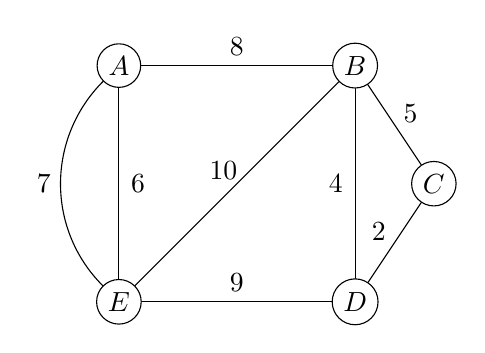
\begin{tikzpicture}[line cap = round, line join = round,scale=1]
			\tikzstyle{vertex}=[circle,draw,minimum size=12pt,inner sep=2pt]
			\foreach \d/\x/\y in {A/0/0, B/3/0, C/4/-1.5, D/3/-3, E/0/-3} {\node[vertex] (\d) at (\x,\y) {$\d$};}
			\foreach \a/\b/\l in {A/B/8, B/C/5, C/D/2, D/B/4, D/E/9, E/B/10, A/E/6} {\draw (\a)-- node [midway,sloped,above] (L){\phantom{L}} (\b); \node at (L) {$\l$};}
			\draw (A) to[out=-135, in=135] node [midway,left] {$7$} (E);
		\end{tikzpicture}}
	\shortans{39}
	\loigiai{
		Quãng đường người đưa thư đi từ $A$ đến $D$ là: $7+6+10+4+8+5+2+9=51$\\
		Quãng đường ngắn nhất đi từ $D$ về $A$ là qua $B$ : $4+8=12$\\
		Tổng quãng đường người đưa thư có thể đi ngắn nhất có thể là: $51+12=63$ .}
	\loigiai{
		Đi từ $C$ đến $E$ theo đường đi Euler dài: $2+1+4+3+5+6+10=31$ (km)\\
		Đi từ $E$ đến $C$ với quảng đường ngắn nhất dài: $5+1+2=8$ (km)\\
		Vậy tổng số kilomet mà người đưa thư phải đi nhỏ nhất là $31+8=39$ (km)}
\end{ex}
\begin{ex}%Câu 19
	Cho một tấm nhôm hình lục giác đều cạnh $90$ cm. Người ta cắt ở mỗi đỉnh của tấm nhôm hai hình tam giác vuông bằng nhau, biết cạnh góc vuông nhỏ bằng $x$ (cm) (cắt phần tô đậm của tấm nhôm) rồi gập tấm nhôm như hình vẽ để được một hình lăng trụ lục giác đều không có nắp. Tìm x để thể tích của khối lăng trụ lục giác đều trên là lớn nhất.\\
	\centerline{\includegraphics[width=.7\textwidth]{images/3.19}}
	\shortans{15}
	\loigiai{
	% {\color{red}HÌNH Ở ĐÂY}\\
	Điều kiện $0<x<45$\\
	Cạnh đáy của lăng trụ lục giác đều:$AB=HK=90-2x$\\
	Chiều cao của lăng trụ lục giác đều: $HA=MH.\tan 60^\circ=x\sqrt{3}$\\
	Diện tích đáy của lăng trụ lục giác đều: $S_{ABCDEF}=6S_{ABO}=6.\dfrac{\sqrt{3}}{4}{\left(90-2x\right)^2}=9x(45-x)^2$\\
	Thể tích của khối lăng trụ lục giác đều: $V(x)=HA.S_{ABCDEF}=9x\left(45-x\right)^2$\\
	Hay $V(x)=9x\left(45-x\right)^2$\\
	Xét hàm số $V(x)=9x\left(45-x\right)^2$ trên khoảng $\left(0;\,45\right)$.\\
	Bảng biến thiên:
	\begin{center}
		
\begin{tikzpicture}
			\tkzTabInit[lgt=1.2,espcl=2]
			{$x$ /.7, $V’(x)$ /.7, $V(x)$ /2}
			{$-\infty$,$15$,$45$,$+\infty$}
			\tkzTabLine{ ,+,z,-,z,+, }
			\tkzTabVar{-/$-\infty$,+/$V(15)$,-/$V(45)$,+/$+\infty$}
		\end{tikzpicture}
	\end{center}
	Từ bảng biến thiên ta có: $\max \limits_{(0;45)}V(x)=V(15)=243000$ (cm$^3$)\\
	Vậy thể tích của khối lăng trụ lục giác đều lớn nhất khi và chỉ khi $x=15$ cm}
\end{ex}
\begin{ex}%Câu 20
	Từ một quả cầu bằng đá trắng sứ bán kính bằng 1 dm, người ta khoan rút lõi ngay \lq\lq chính giữa\rq\rq~ quả cầu (trục đối xứng của lõi và quả cầu trùng nhau) như hình sau với đường kính mũi khoan là 1 dm được một vật thể có thể tích $V$ là bao nhiêu dm3? (Bỏ qua độ dày mũi khoan và kết quả làm tròn đến chữ số thập phân thứ hai sau dấu phẩy)\\
	\centerline{
		\includegraphics[width=.2\textwidth]{images/3.20a.png}
		\includegraphics[width=.25\textwidth]{images/3.20b.jpg}
		\includegraphics[width=.25\textwidth]{images/3.20c.png}
	}
	\shortans{1,47}
	\loigiai{
	Gọi $V_1$ là thể tích của khối trụ và $V_2$ là thể tích của chỏm cầu\\
	Nửa chiều cao của khối trụ là: $l=\sqrt{1^2-\left(0,5\right)^2}=\dfrac{\sqrt{3}}{2}$ nên ta có thể suy ra chiều cao của chỏm cầu là: $h=1-\dfrac{\sqrt{3}}{2}$ . Thể tích khối trụ là: $V_1=\pi{R^2}.H=\pi .R^2.2l=\dfrac{\pi\sqrt{3}}{4}$\\
	Thể tích chỏm cầu: $V_2=\pi\displaystyle\int\limits_{R-h}^R{\left(\sqrt{R^2-x^2}\right)^2dx}$ $\Leftrightarrow{V_2}=\pi\displaystyle\int\limits_{R-h}^R{\left(R^2-x^2\right)dx\Leftrightarrow{V_2}=\,}\pi\left.\left(R^2x-\dfrac{x^3}{3}\right)\right|_{R-h}^R$\\
	$\Leftrightarrow{V_2}=\pi\left[\left(R^3-\dfrac{R^3}{3}\right)-\left(R^2\left(R-h\right)-\dfrac{\left(R-h\right)^3}{3}\right)\right]$ $\Leftrightarrow{V_2}=\pi{h^2}\left(R-\dfrac{h}{3}\right)$ .\\
	Thay số ta suy ra được thể tích của chỏm cầu là $V_2=\pi\left(\dfrac{2}{3}-\dfrac{3\sqrt{3}}{8}\right)$\\
	Khi đó thể tích của khối cần tìm là $V=V_1+2V_2=\dfrac{\pi\sqrt{3}}{4}+\pi\left(\dfrac{2}{3}-\dfrac{3\sqrt{3}}{8}\right)=\dfrac{8-3\sqrt{3}}{6}\pi\approx 1,47$ dm3}
\end{ex}
\begin{ex}%Câu 21
	Sân hiên hình chữ nhật của một ngôi nhà là khoảng đất $ABCD$ được lợp mái bằng kính màu để hạn chế ánh sáng đi qua với mái dốc. Các bề mặt bên $ADHE$ và $CGHD$ nằm ở bức tường bên ngoài ngôi nhà. Đặt vào mô hình hệ trục tọa độ như hình vẽ thì ta có $B\left(5;\dfrac{7}{2};0\right)\,;\,\,E\left(5;0;2\right)$ và $H\left(0;0;3\right)$ . Trên tường nhà có một ngọn đèn đặt tại điểm $L$ cách điểm $D$ một khoảng $6$ m theo phương thẳng đứng. Phần có mái của sân hiên in bóng lên khu vườn bằng phẳng phía trước ngôi nhà dưới ánh đèn tạo thành khoảng đất hạn chế ánh sáng. Tính diện tích khoảng đất đó (Kết quả làm tròn kết quả đến hàng phần chục).
	\shortans{45,9}
	\loigiai{
	{\color{red}HÌNH Ở ĐÂY}\\
	Ta có $H$ là trung điểm của $DL$ nên $GH$ là đường trung bình của $\Delta LD{G}'$ nên ta suy ra $G$ là trung điểm của $L{G}'$ .\\
	Mặt khác: $GC$ là đường trung bình của $\Delta LD{G}'$ nên $G'\left(0;\,7\,;0\right)$\\
	Ta có: $\dfrac{E'A}{ED}=\dfrac{EA}{LD}=\dfrac{2}{6}=\dfrac{1}{3}\Rightarrow{E}'A=\dfrac{1}{3}{E}'D\Rightarrow{E}'A=\dfrac{1}{2}AD=2,5\Rightarrow{E}'\left(7,5;0 ;0\right)$\\
	Mặt khác: $\dfrac{EF}{E'{F}'}=\dfrac{LE}{L{E}'}=\dfrac{2}{3}\Rightarrow{E}'{F}'=1,5.EF=1,5.3,5=5,25$\\
	Diện tích khoảng đất khi đó là: $S_{DG'F'E'}=\dfrac{\left(DG'+E'F'\right).DE'}{2}=\dfrac{(7+5,25).7,5}{2}=45,9$
	}
\end{ex}
\begin{ex}%Câu 22
	Có hai chiếc hộp, hộp I có $5$ viên bi màu trắng và $5$ viên bi màu đen; hộp II có $6$ viên bi màu trắng và $4$ viên bi màu đen. Các viên bi có cùng kích thước và khối lượng. Lấy ngẫu nhiên đồng thời hai viên bi từ hộp I bỏ sang hộp II. Sau đó lấy ngẫu nhiên một viên bi từ hộp II. Lấy ra ngẫu nhiên một viên bi, giả sử viên bi được lấy ra là viên bi màu trắng. Tính xác suất viên bi màu trắng đó thuộc hộp I (Kết quả làm tròn $2$ chữ số thập phân)
	\shortans{0,14}
	\loigiai{
		Xét các biến cố: $A$ : \lq\lq Viên bi lấy ra là viên màu trắng\rq\rq~\\
		$B_1$ : \lq\lq 2 viên bi lấy ra từ hộp I có màu trắng\rq\rq~; $B_2$ : \lq\lq 2 viên bi lấy ra từ hộp I có màu đen\rq\rq~.\\
		$B_3$ : \lq\lq 2 viên bi lấy ra từ hộp I có cả hai màu đen trắng\rq\rq~.\\
		Ta có: $P\left(B_1\right)=\dfrac{\text{C}_5^2}{\text{C}_{10}^2}=\dfrac{2}{9};\,\,P\left(B_2\right)=\dfrac{\text{C}_5^2}{\text{C}_{10}^2}=\dfrac{2}{9};\,P\left(B_3\right)=\dfrac{\text{C}_5^1\cdot\text{C}_5^1}{\text{C}_{10}^2}=\dfrac{5}{9}.$\\
		Áp dụng công thức xác suất toàn phần, ta có\\
		$P(A)=P\left(A|B_1\right).P\left(B_1\right)+P\left(A|B_2\right).P\left(B_2\right)+P\left(A|B_3\right).P\left(B_3\right)$ $=\dfrac{8}{12}.\dfrac{2}{9}+\dfrac{6}{12}.\dfrac{2}{9}+\dfrac{7}{12}.\dfrac{5}{9}=\dfrac{7}{12}$\\
		Gọi $C$ là biến cố: \lq\lq Viên bi lấy ra là bi trắng từ hộp I\rq\rq.\\
		Khi đó ta có:\\
		$P(C)=P(C|B_1).P(B_1)+P(C|B_2).P(B_2)+P(C|B_3).P(B_3) = \dfrac{2}{12}. \dfrac{2}{9}+0.\dfrac{2}{9}+\dfrac{1}{12}.\dfrac{5}{9}=\dfrac{1}{12}$.\\
		Vậy xác suất cần tìm là:\\ 
		$P\left(C|A\right)=\dfrac{P(CA)}{P(A)}=\dfrac{\dfrac{1}{12}}{\dfrac{7}{12}}=\dfrac{1}{7}\approx 0,14 $ (vì $C \subset A$)\\
		}
\end{ex}
\Closesolutionfile{ans}
\Closesolutionfile{ansbook}
\inputansbox{6,2,3}{ans/ans-3-T,ans/ans-3-TF,ans/ans-3-SA}